\documentclass[conference]{IEEEtran}
\IEEEoverridecommandlockouts
% The preceding line is only needed to identify funding in the first footnote. If that is unneeded, please comment it out.
% \usepackage{cite}
\usepackage{amsmath,amssymb,amsfonts}
\usepackage{algorithmic}
\usepackage{graphicx}
\usepackage{hyperref}
\usepackage{textcomp}
\usepackage{xcolor}
\usepackage{fancyhdr}
\usepackage{longtable}

\def\BibTeX{{\rm B\kern-.05em{\sc i\kern-.025em b}\kern-.08em
    T\kern-.1667em\lower.7ex\hbox{E}\kern-.125emX}}
    
% ANCS'19 Conference Name 

%Set the font (output) encoding
\usepackage[T1]{fontenc} 

%Portuguese-specific commands
% \usepackage[portuguese]{babel}

%Hyphenation rules
\usepackage{hyphenat}
\hyphenation{mate-mática recu-perar}

%%%%%%%%%%%%%%%%%%%%%%%%%%%%%%%%%%%%%%%%%%%%%%%%%%%%%%%%%%%%%%%%
\chead{\rmfamily\fontsize{9}{30}\selectfont 
Professional Master's Degree - Graduate Program in Applied Computing (PPCA) - UnB - Discipline Data Mining - june/2023}
\renewcommand{\headrulewidth}{0pt}
%%%%%%%%%%%%%%%%%%%%%%%%%%%%%%%%%%%%%%%%%%%%%%%%%%%%%%%%%%%%%%%%%%%%%%%%%%%%%%%%%%%%%%%%%%

% ANCS'19 Copyright Notice %%%%%%%%%%%%%%%%%%%%%%%%%%%%%%%%%%%%%%%%%%%%%%%%%%%%%%%%%%%%%%%%%%%%%%%%%%%%%%%%%%%%%%%%%%%%%%%%%
% Note: use the copyright text that matches your requirements.
% For all other papers the copyright notice is:
\cfoot{\rmfamily\fontsize{9}{0}\selectfont 978-1-7281-4387-3/19/\$31.00~\copyright~2019 IEEE}
%%%%%%%%%%%%%%%%%%%%%%%%%%%%%%%%%%%%%%%%%%%%%%%%%%%%%%%%%%%%%%%%%%%%%%%%%%%%%%%%%%%%%%%%%%%%%%%%%%%%%%%%%%%%%%%%%%%%%%%%%%%%%

% Pacote abnt-biblatex
\usepackage[style=abnt]{biblatex}
\usepackage{array}
\usepackage{tabularx}
\usepackage{mwe}
\usepackage{float}
\usepackage{adjustbox}
\usepackage{graphicx}

\addbibresource{MD Exercício 2.bib}      
\begin{document}

\title{Prioritization of Government Auditing by Ranking: A Case Study Using Health, Education and Public Security Data from Distrito Federal's Administrative Regions \\
% \title{Priorização de Auditorias no DF por ranqueamento: Um estudo de Caso usando dados de Saúde, Educação e Segurança Pública das Regiões Administrativas\\
{\footnotesize \textsuperscript{}}
\thanks{}
}




\author{\IEEEauthorblockN{1\textsuperscript{st} Augusto Nunes}
\IEEEauthorblockA{\textit{ student discipline MD/PPCA } \\
\textit{UnB}\\
Brasília, Brazil \\
augcrn@gmail.com}
\and
\IEEEauthorblockN{2\textsuperscript{nd} Ennio Ferreira}
\IEEEauthorblockA{\textit{student discipline MD/PPCA} \\
\textit{UnB}\\
Brasília, Brazil \\
ennioferreirab@gmail.com}
\and
\IEEEauthorblockN{3\textsuperscript{rd} Mayra Campos}
\IEEEauthorblockA{\textit{student discipline MD/PPCA} \\
\textit{UnB}\\
Brasília, Brazil \\
mayra.campos@gmail.com}
}

\maketitle
\thispagestyle{fancy}


% Augusto: Vou alterar o Abstract porquê a gente não tá usando só dado do Portal da Transparência do DF, mas sim dados abertos de maneira mais geral
\begin{abstract}
In this study we present a novel indicator that could be used in the annual planning phase of internal government auditing done by the executive branch of Distrito Federal's executive government branch responsible for internal auditing, the Comptroller-General of Distrito Federal \textit{Controladoria-Geral do Distrito Federal}. Using open data in four dimensions (vulnerabilites): health, education, sociodemographic and public security, by clustering the 33 Administrative Regions into 06 clusters using unsupervised K-Means and ranking a subset of the variables that an internal auditor chose, we were able to suggest an indicator that achieved high concordance - 90\% in general and 70\% \textit{intra} cluster - when evaluated against the 2022 internal auditing reports.
% Este é o artigo final do projeto que será apresentado para a disciplina Miueração de Dados, ministrada no 1o Semestre de 2023 pelo Prof. Dr. Marcelo Ladeira no Mestrado Profissional em Computação Aplicada da Universidade de Brasília. Utilizamos conjuntos de dados abertos disponíveis no “Portal da Transparência do Distrito Federal”, bem como de outras fontes abertas tais como  o Datasus, e-Gestor AB e INEP para adaptar o trabalho feito por \{nascimento_indice_2022} para o contexto do controle interno feito pela Controladoria-Geral do Distrito Federal.
\end{abstract}

\begin{IEEEkeywords}
data mining; internal auditing; risk-based auditing; cluster analysis; ranking statistics
% mineração de dados; dados abertos; controle interno;  auditoria baseada em riscos;  ciência de dados
\end{IEEEkeywords}

\section{Introduction}
\subsection{Context Description}
The Comptroller-General of Distrito Federal (CGDF) has, among its institutional attributions, "to secure good and regular application of public resources, and to coordinate the internal control system of the executive government branch"\footnote{Translated from \url{https://www.cg.df.gov.br/competencias-2/}}. These institutional assignments unpack not only in the most direct actions on fraud detection and the enforcement on governance controls among all executive branches to reduce its risk, but also on asserting that ideally all of the public sector planning, decisions and activities are mindful of the stakeholders interest in the public and private sectors. 

In order to assert that these attributions are carried out, one of the actions that are periodically executed are plannings of audits to be done by the internal auditors teams of CGDF at the end of each first semester of the year. These planning phases the longer term auditing processes that will be carried out for the next 12 months, directing the auditing efforts toward those that have the \textit{biggest potential} for generating societal return. Furthermore, the audits are also carried when there are facts of general commotion reported in the media or when any irregular acts come to the knowledge of the auditors, usually by complaints made within the ombudsman service.

There are many approaches for evaluating which audits could have this biggest potential impact, and for ranking them having in mind that internal audits can't reach every single government action, either because there's scarcity of resources or because the expected return of an expensive auditing process would be minimal. One of those uses the discipline of \textit{Risk-based auditing}, as established in the Internal Audit Capability Model (IA-CM) for the Public Sector framework. 

Risk is anything that could lead to the objectives not being achieved. In this context, we can understand \textit{risk} as both the risk that the government endeavour which is under scrutiny of the internal auditors did not meet its objectives, and as the risk of the relative success of the auditing process itself. This work mainly focuses on the first interpretation, which is to suggest by looking at some variables associated with the Administrative Regions of the Federal District we will be able to propose an index that will be capable to capture which of the Administrative Regions have citizens in general at a higher risk, and thus which of those Administrative Regions should receive precedence in the internal audits. 

Risks vary in nature, some are very direct, such as the materiality of the endeavour - i.e. the amount of money the government spent or is planning to spend to achieve a certain objective - but others are not directly measurable by merely inspecting official documents. The Comptroller-General of the Union, in its Manual of Technical Guidelines for Government Internal Audit Activities\footnote{Available in Portuguese at \url{https://wiki.cgu.gov.br/index.php/Manual_de_Orienta\%C3\%A7\%C3\%B5es_T\%C3\%A9cnicas_da_Atividade_de_Auditoria_Interna_Governamental_do_Poder_Executivo_Federal}}, uses two categories for risk assessment: quantitative and qualitative. It states that qualitative risks have a certain degree of subjectivity, and exemplify them by referencing the social impact that is associated with an audit object. 

\subsection{Problem}

The Federal District has both Brazil's highest GDP \textit{per capita} in one of its Administrative Regions, \textit{Lago Sul}; and the country's biggest \textit{favela} in another, \textit{Sol Nascente}. Such discrepancies in the geographic and social space are to blame for many side effects of economic inequality, as stated by \cite{pattussi2001social}, \cite{azzoni2002education} and \cite{sachsida2010inequality}. Even though these works are not focused on the problem of internal auditing, this suggests the inequality of access to basic needs poses a strong risk to the success of government endeavours in areas were it is most rampant.

In this work, we use a set of variables that lie in four dimensions - thus called \textit{vulnerabilites} - of public policy evaluation, namely health, education, sociodemographic and public security, all of these freely available according to the discipline of open data, and we propose an index based on the qualitative risk attributed in these four vulnerabilities that could be used in the planning phase of the annual internal audits carried by the institution for the general composition of the 33 Administrative Regions that the Federal District currently has, and also on 6 clusters which were identified using the unsupervised K-Means algorithm. The clustering analysis also provides some insight into the compositional similarities between those administrative regions, identifying those which are at higher risk.

% Neste trabalho, utilizaremos um subconjunto dos 33 fatores representativos do Índice de Priorização de Objetos de Auditoria (IPOA) elencados por \cite{nascimento_indice_2022} no contexto da Controladoria-Geral da União, em particular para os municípios do estado de Sergipe,  para avaliar sua aplicabilidade ao contexto do Distrito Federal, em particular no planejamento das auditorias realizadas pela Controladoria-Geral do Distrito Federal nas Regiões Administrativas. 

% Um dos resultados esperados por esse trabalho é a avaliação da aplicabilidade deste subconjunto dos fatores propostos originalmente, e que lá foram sugeridos como aplicáveis no contexto mais geral da Controladoria-Geral da União. Uma das tarefas cruciais é tentar \textit{traduzir} o contexto dos municípios do estado de Sergipe para as Regiões Administrativas do Distrito Federal, levando em conta as discrepâncias formais e administrativas entre estes dois entes. 

% Para além disso, a própria composição do IPOA sugere uma possibilidade de diagnóstico socioeconômico, de saúde e de educação que pode ser importante não apenas no planejamento das auditorias mas também como ferramenta de diagnóstico de fragilidades pelo governo distrital, notando para quais Regiões Administrativas observamos valores piores para os fatores de composição do indicador.

% \section{Context Description and Problem}

\section{Literature Review}

Generally speaking, the Institute of Internal Auditors (IIA) is the \textit{de facto} authority regarding auditing activities both in private and public sectors. Internal auditing in public agencies and more generally government activities is most often treated as a separate practice from the private internal auditing, given its nuanced list of priorities and obligations which are not fundamental in private settings. 

The most reputable reference published by the IIA is the Internal Audit Capability Model (IA-CM) for the Public Sector: Overview and Application Guide \cite{institute_of_internal_auditors_internal_2009}. This publication proposes an assessment framework for the phases of an internal audit in the governmental perspective, using the idea of Key Performance Areas (KPA) as a series of stepping stones for the internal auditors working in the public sector. None of these KPA have an approach that considers the vulnerabilites here studied.

We investigated reputable references that deal with the problem of prioritization of public government auditing, and concluded that many of these deal primarily with the auditing processes limited to the financial (i.e fraud, waste or collusion) perspective of materiality as the majoring factor in assessing risk. 

\textcite{balaniuk2012risk} considered the use of a Naïve Bayes classifier trained on data pertaining to the purchases effected by the Federal Government, using variables related both to the executive branch of the government that ordered the purchase and the private entity that participated in the process. They proposed the classifier as a semi-automated risk assessment framework capable of mitigating the inherent financial menaces associated with these activities. So, even though this work utilises a classic approach in Data Mining, it falls short to address anything remotely close to what we propose here, instead focusing on the official documentation produced in the formal processes of government purchasing and later accounting reviews as the predictors of whether a similar process might also be fraudulent.

One interesting source we consulted was the work of \textcite{nascimento_indice_2022}: in his monograph he proposed an approach similar to the one we have chosen here, but applied it for the Brazilian state of Sergipe and its municipalities. It also uses the novel approach of considering dimensions and variables for risk assessing in the planning phase other than the typical object measures that are more often employed in financial internal auditing. Even though this is a similar work, we could not merely translate this work to the context of the Federal District, given that it is not exactly the same as municipalities in other states of Brazil in terms of constitutional law. We tried to circumvent this limitation treating the Administrative Regions as \textit{municipalities}, but this also has the shortcoming that they are not, as stated in the organic law.

% \begin{enumerate}
%     \item a primeira linha realizada dentro da própria unidade, pelos servidores públicos responsáveis pelos processos de execução, monitoramento e avaliação;
%     \item a segunda incumbe-se das tarefas de gestão dos riscos associados aos procedimentos da primeira linha, sendo também realizada por servidores da própria unidade de execução;
%     \item e a terceira linha, realizada pela Controladoria-Geral do Distrito Federal (CGDF) e por essência independente da unidade executora das ações, que tem por objetivo reportar os achados de auditoria à alta administração das unidades e do governo local, bem como publicizá-los quando consolidados.
% \end{enumerate}
   

% Esta abordagem sugere que as ações de controle ocorrem de maneira sucessiva, e que as duas primeiras linhas são responsáveis por mitigar os riscos inerentes às despesas, contratações e demais atos da administração pública que por ventura possam ferir os princípios listados no artigo 37 da Constituição Federal da República Federativa do Brasil. Caso estas falhem, aí sim o controle-interno é impelido a agir. No entanto, há um vácuo entre a necessidade de ação e a efetiva ação dos auditores. 

% Uma das maneiras de reduzir esse vácuo de ação estabeleceu-se na disciplina conhecida como Auditoria Baseada em Riscos (\textit{Risk Based Auditing}), que em \textit{lato sensu} impõe às organizações uma série de medidas fundamentadas no gerenciamento do risco, tendo sido inclusive firmada como a norma ISO 31000/2018. A Auditoria Baseada em Riscos deve, por premissa, focar suas ações e recomendações prioritariamente nos contextos que apresentam maior risco, onde \textit{risco} é tudo aquilo que pode ter impacto nos objetivos da organização. 

% Surge então a necessidade de mensurar os riscos inerentes às ações da administração pública. Em seu trabalho de conclusão de curso, \textcite{nascimento_indice_2022} sugere a criação de um Índice de Priorização de Objetos de Auditoria (IPOA) no contexto da Controladoria-Geral da União. O IPOA é \textit{"(...)um modelo matemático-estatístico que agrupa e prioriza municípios, estados, programas ou ações governamentais com base em fatores de risco previamente determinados"}, e foi desenvolvido de maneira preliminar pelo autor apenas com dados referentes aos municípios do estado de Sergipe. A composição do indicador se deu através da análise de quatro dimensões, ditas \textit{vulnerabilidades}: à \textbf{fraude}; na atenção primária da \textbf{saúde}; na \textbf{educação} básica; e \textbf{socioeconômica}.

% Surge então a necessidade de mensurar os riscos inerentes às ações da administração pública. Em seu trabalho de conclusão de curso, \textcite{nascimento_indice_2022} sugere a criação de um Índice de Priorização de Objetos de Auditoria (IPOA) no contexto da Controladoria-Geral da União. O IPOA é \textit{"(...)um modelo matemático-estatístico que agrupa e prioriza municípios, estados, programas ou ações governamentais com base em fatores de risco previamente determinados"}, e foi desenvolvido de maneira preliminar pelo autor apenas com dados referentes aos municípios do estado de Sergipe. A composição do indicador se deu através da análise de quatro dimensões, ditas \textit{vulnerabilidades}:
% \begin{itemize}
%     \item à \textbf{fraude};
%     \item na atenção primária da \textbf{saúde};
%     \item na \textbf{educação} básica;
%     \item e \textbf{socioeconômica}.
% \end{itemize}

% \begin{figure}[htbp]
% \centerline{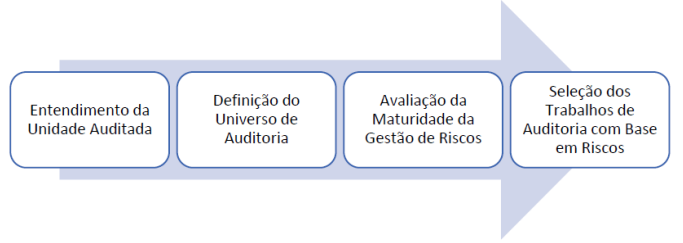
\includegraphics[scale=0.6]{procCGU.png}}
% \caption{Processo de Planejamento da Unidade de Auditoria Interna Governamental - Fonte: SFC/CGU.}
% \label{fig}
% \end{figure}


\section{Methodology}
\subsection{Framework}
For this work we followed what is proposed in the Cross Industry Standard Process for Data Mining, CRISP-DM, in particular the first five of its six phases:

\begin{itemize}
    \item Business Understanding
    \item Data Understanding
    \item Data Preparation
    \item Modeling
    \item Evaluation
\end{itemize}

The first topic is situated here in the Introduction section of this paper, the following three are contained in this Methodology section, and the end we present our findings as the Evaluation. As the nature of this work is mainly speculative, we were unable to apply the sixth phase, Deployment.

% Para o presente trabalho utilizaremos a metodologia CRISP-DM (Cross Industry Standard Process for Data Mining), em português, “Processo Padrão Inter-Indústrias para Mineração de Dados”.

% \begin{figure}[htbp]
% \centerline{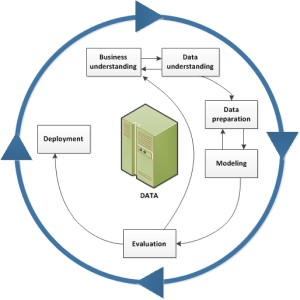
\includegraphics{crisp_process_smaller.jpg}}
% \caption{Ciclo CRISP-DM.}
% \label{fig}
% \end{figure}


% \begin{itemize}
%     \item Compreensão do domínio,  
%     \item Preparação e Compreensão dos dados,
%     \item Modelagem,
%     \item Avaliação 
%     \item Aplicação.

% \end{itemize}

\subsection{Data Understanding}

% Determinação dos objetivos da aplicação: O \textbf{cenário} escolhido é "o planejamento das auditorias baseado em vulnerabilidade social". 

% Os \textbf{Objetivos da aplicação} "agrupar índicadores sociais formando um indice que possibilite facilmente revelar as vulnerabilidades sociais presentes na Região administrativa". 

% Os \textbf{Critérios de sucesso da aplicação} seriam "a otimização do processo de planejamento das auditorias no Governo do Distrito Federal".

% \textbf{Inventário de Recurso} determinamos "a utilização de dados fornecido pelas plataformas e pesquisas publicas.  

\begin{table*}[h]
\small
\centering
\begin{tabularx}{\textwidth}{|l|l|X|}
\hline
\textbf{Source} & \textbf{Variable} & \textbf{Description} \\
\hline
District Domicile Survey & SE1 & Literacy level of the voters (used as a proxy of the proportion of all the population that finished at least high school) \\
\cline{2-3}
 & SE2 & Proportion of families living in extreme poverty (R\$ < 200) that receive social benefits (\textit{Bolsa Família, BPC/Loas} or scholarships)\\
\hline
Datasus & S1 & Rate of fetal mortality (per thousand born alive) \\
\cline{2-3}
 & S2 & Rate of mortality by avoidable causes (per 10,000 inhabitants)\\
\hline
Public Security Secretary & SEG1 & Rate of occurrence of crimes against property (per 1,000 inhabitants)\\
\hline
District School Census & E1 & Student Average per class in elementary school\\
\cline{2-3}
 & E2 & Age-grade lag rate in elementary school \\
\cline{2-3}
 & E3 & Failure rate in elementary school\\
\hline
\end{tabularx}
\caption{Source, code and description of the variables}
\label{tab:variaveis}
\end{table*}

These variables were chosen in discussions with one of the internal auditors of CGDF, and each of them have the same weight in the final indicator according to the opinion of this expert. 

Ideally, we would have 33 observations of the 8 variables described in \ref{tab:variaveis}, one for each of the Administrative Regions of the Federal District, but due to the varying nature of the sources used and the fact that some of the Administrative Regions have only been established very recently, we have a few instances of missing data, which will be imputed as described in the next subsection.
% \begin{table*}[h]
% \small
% \centering
% \begin{tabularx}{\textwidth}{|l|l|X|}
% \hline
% \textbf{Origem} & \textbf{Variável} & \textbf{Descrição} \\
% \hline
% PDAD & SE1 & Grau de instrução dos eleitores do Brasil. Proporção da população com ensino médio ou mais concluído \\
% \cline{2-3}
%  & SE2 & Proporção de famílias em situação de pobreza (R\$ < 200) que recebe benefícios sociais (Bolsa-família, BPC/LOAS, Bolsa de estudo) \\
% \hline
% Datasus & S1 & Taxa de mortalidade fetal (por mil nascidos vivos) \\
% \cline{2-3}
%  & S2 & Taxa de mortalidade por causas evitáveis (por 10.000 habitantes) \\
% \hline
% SSP-DF & SEG1 & Taxa de ocorrências de crimes e delitos registrados pela CCP (por 1.000 habitantes) \\
% \hline
% Censo Escolar DF & E1 & Média de alunos por turma no ensino fundamental \\
% \cline{2-3}
%  & E2 & Taxa de defasagem idade-série no ensino fundamental \\
% \cline{2-3}
%  & E3 & Taxa de reprovação no ensino fundamental \\
% \hline
% \end{tabularx}
% \caption{Tabela das variáveis utilizadas}
% \label{tab:variaveis}
% \end{table*}


% Sendo os \textbf{Requisitos, suposições e limitações} 

% "A origem jurídica e monetária das regiões administrativas do Distrito Federal diferem dos Municípios. Por ser um enti administrativo diferente do padrão, e o pagamento dos custos dos projetos utilizarem dinheiro da União dificulta as análises demográficas e fiscais. A maioria dos estudos federais tratam as Regiões Administrativas como uma unidade única sem detalhes granulares.". 


% Os \textbf{Custos e Benefícios} previstos "Melhorar o planejamento das auditorias fornecendo a visão de quais RAs estão divergindo dos valores médios dos indicadores de vulnerabilidade social. Portanto, indicar as regiãos que estão mais deficitárias socialmente tornando contratos com impacto direto nessas regiões como prioritários quanto a supervisão".

% Sendo os \textbf{Critérios de sucesso} se os especialistas responsáveis pelo planejamento das auditorias atestem que os indicadores sociais revelem quais RAs estão mais vulneráveis e necessitam de maior atenção".

\subsection{Data Preparation}
\begin{itemize}
    \item Standardization of variables: the scale chosen for each of the variables changes according to its interpretation and variability. In order to standardize the behaviour and maintain the most information about their location and scale properties we chose to use z-score normalization.

    \item Interpretation of variable SE1: in order to obtain an indicator that has the interpretation of risk, i.e. higher = most at risk, we chose to multiply SE1 by (-1), with the understanding 

    
    \item Data imputation: some of the smaller Administrative Regions or those created more recently have missing data for some of the attributes. To impute this data, we used Ridge Regression as implemented in the \texttt{IterativeImputer} class of \texttt{scikit-learn}: each of the variables with missing values is treated as a feature in a Ridge Regression, and this process is repeated iteratively at most 10 times.
% \begin{itemize}

% \item Padronização dos indicadores: A escala adotada em cada indicador vária quanto a escala e a variábilidade. A fim de padronizar mantendo a distância de cada indicador à média, e a variabilidade, foi utilizada a normalização.

% \item Imputação de dados faltantes: Algumas RAs menores não coletam algumas variáveis. Para os dados faltantes, foi utilizada a técnica de imputação em que foi treinado um modelo de regressão ridge predizendo o dado faltante utilizando as demais colunas como dependente.

\begin{table}
\centering
\begin{tabular}{|c|c|}
\hline
\textbf{Administrative Region} & \textbf{Attributes with missing data} \\
\hline
Candangolândia & SEG1 \\
\hline
Sudoeste/Octogonal & SEG1 \\
\hline
Park Way & SEG1 \\
\hline
Sobradinho II & E3 \\
\hline
Jardim Botânico & E3 \\
\hline
Itapoã & E3 \\
\hline
SIA & S2, SE2 \\
\hline
Vicente Pires & E3 \\
\hline
Fercal & E1, E2, E3 \\
\hline
Sol Nascente/Pôr do Sol & S1, S2, E1, E2, E3 \\
\hline
\end{tabular}
\caption{Administrative Regions and the attributes for which there is missing data}
\label{tab:colunas-NA}
\end{table}
% \begin{table}
% \centering
% \begin{tabular}{|c|c|}
% \hline
% \textbf{Cidade} & \textbf{Colunas NA a serem completadas} \\
% \hline
% Candangolândia & SEG1 \\
% \hline
% Sudoeste/Octogonal & SEG1 \\
% \hline
% Park Way & SEG1 \\
% \hline
% Sobradinho II & E3 \\
% \hline
% Jardim Botânico & E3 \\
% \hline
% Itapoã & E3 \\
% \hline
% SIA & S2, SE2 \\
% \hline
% Vicente Pires & E3 \\
% \hline
% Fercal & E1, E2, E3 \\
% \hline
% Sol Nascente/Pôr do Sol & S1, S2, E1, E2, E3 \\
% \hline
% \end{tabular}
% \caption{Tabela das colunas NA a serem completadas por cidade}
% \label{tab:colunas-NA}
% \end{table}



\item Collinearity: it is not uncommon when studying demographic problems that strong correlations arise in the data, which generally poses itself as a problem for when adjusting models \cite{hill2001collinearity}. In particular, the variables SE1 and SE2 presented a Fisher correlation score of 0.77, but it was a decision of the consulted internal auditor to keep both of these variables in the proposed index. 
% \item Colinearidade: Variáveis sociais são por natureza dependentes entre si. Dentre as variáveis, SE1 e SE2 possuem correlação linear de 0,77, porém por indicação do especialista consultado elas permaneceram no modelo pela importância na segmentação da população mais vulnerável.

\begin{figure}[H]
    \centering
    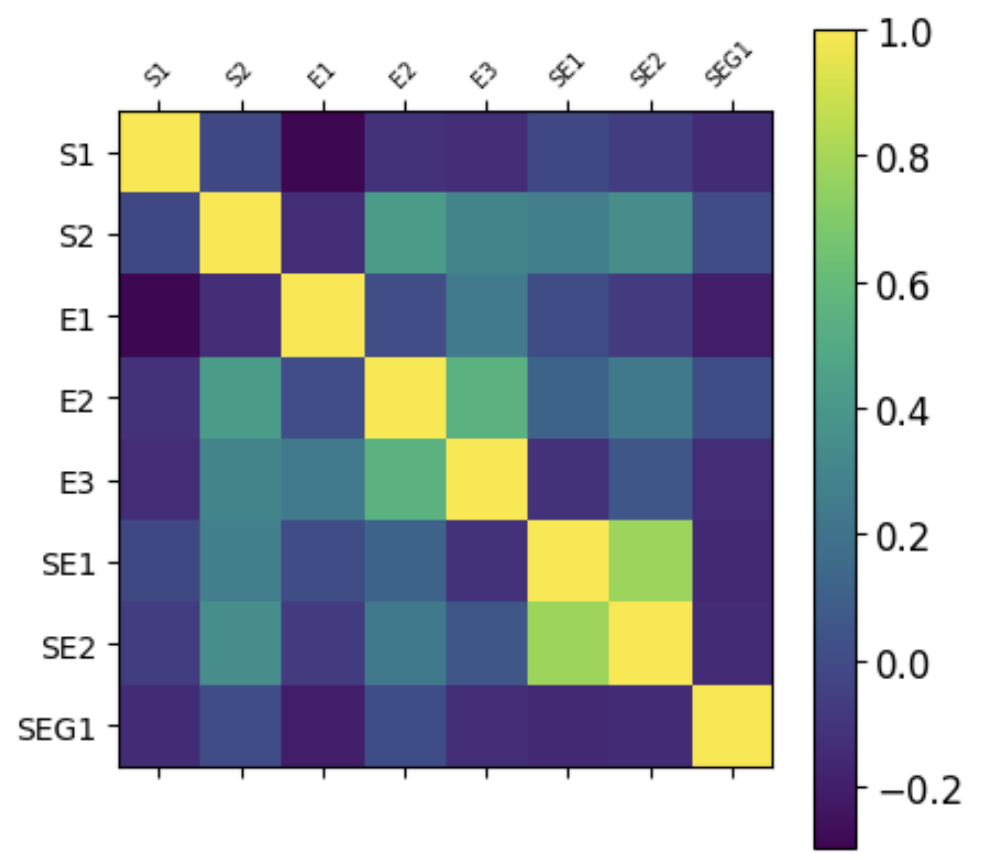
\includegraphics[width=\linewidth]{matriz_correlacao.png}
    \caption{Correlation matrix of the variables post normalization and imputation}
    \label{fig:correlacao}
\end{figure}

\item Definition of the Vulnerability Index: we chose the linear combination of the factors 
% \item Criação do Indice de Vulnerabilidade:

% Foi feita a combinação linear das variáveis. Indicando quanto maior o valor do indice, maior a vulnerabilidade.

\begin{equation}
\text{X}_{\text{index.}} = S1+ S2+ E1+ E2+ E3+ SE1 + SE2+ SEG1
\end{equation}

\end{itemize}

\subsection{Modelling}
\begin{itemize}
\item In order to segment the Administrative Regions by their vulnerability similarity, we used the K-Means clusterization technique, which tentatively separates the Administrative Regions which are most similar inside the same cluster, and put those least similar in different ones.
\item One of the challenges we face when we use K-Means as an unsupervised clusterization technique is to determine the optimal number of clusters. An approach is to calculate the Elbow metric, which uses the concept of internal inertia of the clusters while it computes teh sum of the squared distances from each point to its assigned center, for a range of the tentative number of clusters we choose initially. The Elbow metric for our problem indicated that 6 is the optimal number of clusters, as illustrated in the Figure \ref{fig:parametro_modelo}.

\begin{figure}[H]
  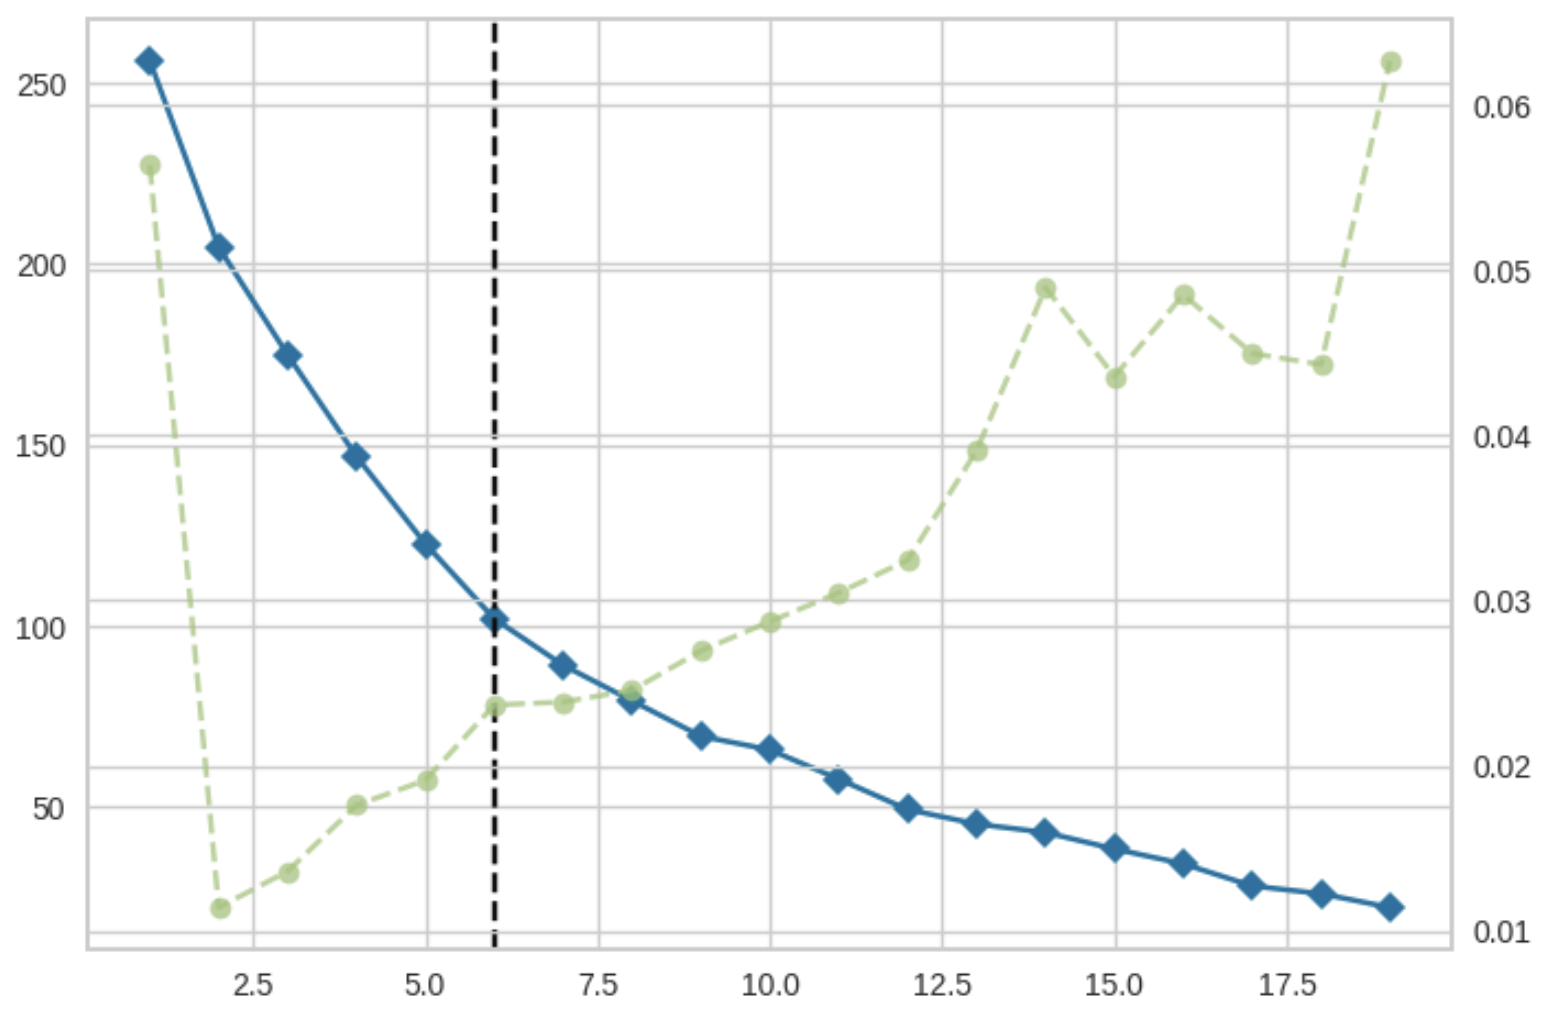
\includegraphics[scale=0.30]{parametro_modelo.png}
  \caption{Métrica Elbow. Quantidade de grupos formados}
  \label{fig:parametro_modelo}
\end{figure}

\end{itemize}
% \begin{itemize}
% \item Com o objetivo de segmentar as regiões administrativas por similaridade de vulnerabilidade, foi utilizada a técnica de clusterização K-Means. O algoritmo cria grupos tentando aumentar a similaridade internamente , ao mesmo tempo que tenta aumentar a distância entre os grupos.
% \item A quantidade de grupos formatos pelo K-Means deve ser selecionado previamente. Foi utilizado a métrica Elbow em que iterativamente vai aumentando a quantidade de grupos e cálculando a inercia interna, enquanto que cálcula a distância entre os grupos. A métrica indica o ponto em que a adição de mais clusters não resulta em maior segmentação. A métrica retornou 6 clusters sendo o número ótimo.

% \begin{figure}[H]
%   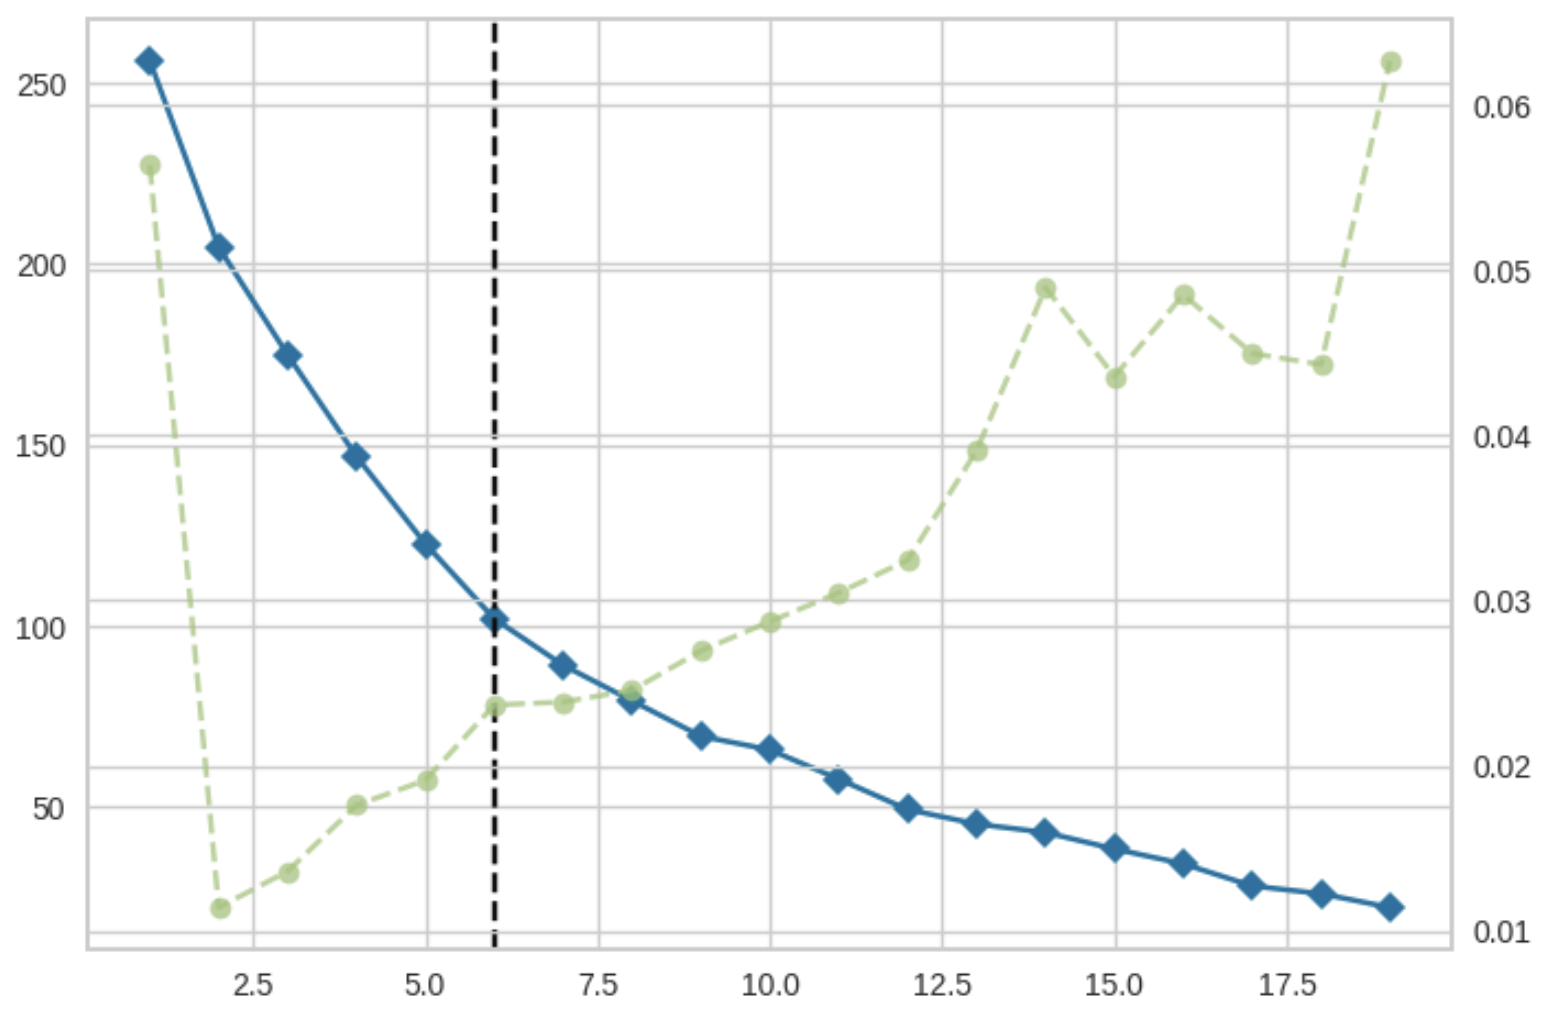
\includegraphics[scale=0.30]{parametro_modelo.png}
%   \caption{Métrica Elbow. Quantidade de grupos formados}
%   \label{fig:parametro_modelo}
% \end{figure}

% \end{itemize}

\section{Evaluation}

Considering the general perspective of Administrative Regions according to the proposed vulnerability index $V_index.$.
% Considerando a visão general das regiões administrativas de acordo com o indice de vulnerabilidade criado.

\begin{table}[H]
\centering
\begin{tabular}{|c|r|}
\hline
\textbf{Administrative Region} & \textbf{Vulnerability Index} \\
\hline
Fercal & 8.712 \\
\hline
SIA & 6.228 \\
\hline
Candangolândia & 5.353 \\
\hline
Sobradinho & 5.353 \\
\hline
SCIA/Estrutural & 5.092 \\
\hline
Planaltina & 4.949 \\
\hline
São Sebastião & 4.393 \\
\hline
Varjão & 4.352 \\
\hline
Ceilândia & 3.055 \\
\hline
Sol Nascente/Pôr do Sol & 3.001 \\
\hline
Brazlândia & 2.663 \\
\hline
Riacho Fundo II & 2.607 \\
\hline
Santa Maria & 2.347 \\
\hline
Itapoã & 2.324 \\
\hline
Park Way & 1.681 \\
\hline
Núcleo Bandeirante & 1.542 \\
\hline
Cruzeiro & 1.281 \\
\hline
Recanto das Emas & 0.954 \\
\hline
Paranoá & 0.907 \\
\hline
Taguatinga & 0.422 \\
\hline
Jardim Botânico & 0.270 \\
\hline
Lago Norte & -0.071 \\
\hline
Samambaia & -0.165 \\
\hline
Gama & -0.469 \\
\hline
Águas Claras & -1.019 \\
\hline
Vicente Pires & -1.173 \\
\hline
Sobradinho II & -1.594 \\
\hline
Lago Sul & -2.121 \\
\hline
Plano Piloto & -2.524 \\
\hline
Guará & -2.830 \\
\hline
Riacho Fundo & -3.059 \\
\hline
Sudoeste/Octogonal & -4.459 \\
\hline
\end{tabular}
\caption{Administrative Regions and their respective Vulnerability Indices, sorted in decreasing order.}
\label{tab:vulnerabilidade}
\end{table}


The proposed ranking makes sense when we look at the socio-economic conditions of some of those that ranked at the top: \textit{Fercal} itself is an Administrative Region which has its roots in rural activites and owe its name to a cement industry, marred with inequality and pollution of air and water, is consistently facing problems regarding access to basic needs, such as infrastructure, job opportunities, and the scarcity of public endeavours in education and public health services \cite{santos2016percepccoes}.

\textit{SIA} is an Administrative Region that originally catered exclusively to the industrial needs of the Federal District, such as the beverage industry and gasoline/diesel silos, but is now being gradually occupied by businesses and residencies. This occupation though is not being accompanied by the public services, particularly in regards to public security vulnerability, as evidenced by its value for the variable SEG1 (rate of occurrence of crimes against property) 5.42, much higher than for the other Administrative Regions. 


At the bottom, we have some Administrative Regions such as \textit{Sudoeste/Octogonal}, \textit{Riacho Fundo} and \textit{Guará}, which in general are better served with public infrastructure such as police departments, basic sanitation and schools.
% O ranking criado parece fazer sentido ao se considerar as condições socioeconômicas e infraestruturais existentes em cada região administrativa. Fercal, SIA e Candangolândia, de acordo com o índice de vulnerabilidade, são as mais vulneráveis. Essas regiões possuem históricos de desafios relacionados à infraestrutura básica, oportunidades de emprego e renda, educação e serviços de saúde.

% Fercal, por exemplo, é uma região de origem rural e que enfrenta dificuldades no que diz respeito à oferta de serviços públicos, como educação, saúde e transporte. SIA, embora seja uma área de importante atividade industrial e comercial, Tem a segurança como ponto critico com a variável SEG1 com o valor de 5.42 indicando a região está muito mais perigosa que a média das demais. Candangolândia, por sua vez, é uma das regiões mais antigas do Distrito Federal e tem a sua maior dificuldade a falta de estrutura para atendimento hospitalar na região.

% No outro extremo do espectro, as regiões administrativas com os menores índices de vulnerabilidade, como Sudoeste/Octogonal, Riacho Fundo e Guará, são geralmente áreas mais bem estruturadas, com melhores condições de vida e acesso a serviços. Isto sugere que o índice de vulnerabilidade criado está de acordo com a realidade sócio-econômica do Distrito Federal



\begin{table}[H]
\centering
\begin{tabular}{|c|c|r|}
\hline
\textbf{Cluster} & \textbf{Administrative Region} & \textbf{Average Vulnerability Index (cluster)} \\
\hline
6 & SIA & 6.228 \\
\hline
5 & Candangolândia & 5.353 \\
 & Fercal &  \\
 & Varjão &  \\
\hline
1 & Brazlândia & 3.055 \\
 & Ceilândia &  \\
 & Itapoã &  \\
 & Planaltina &  \\
 & Riacho Fundo II &  \\
 & SCIA/Estrutural &  \\
 & Sobradinho &  \\
 & Sol Nascente/Pôr do Sol &  \\
 & São Sebastião &  \\
\hline
2 & Cruzeiro & 0.954 \\
 & Jardim Botânico &  \\
 & Núcleo Bandeirante &  \\
 & Paranoá &  \\
 & Park Way &  \\
 & Recanto das Emas &  \\
 & Samambaia &  \\
 & Santa Maria &  \\
 & Taguatinga &  \\
\hline
3 & Gama & -1.384 \\
 & Guará &  \\
 & Lago Norte &  \\
 & Lago Sul &  \\
 & Plano Piloto &  \\
 & Sobradinho II &  \\
 & Vicente Pires &  \\
 & Águas Claras &  \\
\hline
4 & Riacho Fundo & -3.759 \\
 & Sudoeste/Octogonal &  \\
\hline
\end{tabular}
\caption{Groups formed using K-Means and their respective average vulnerability indices}
\label{tab:cidades-cluster}
\end{table}


Using a mere socioeconomic view, the obtained clusters and their average indices provide a very coherent portrait of the disparities between Administrative Regions, and it was able to segment similar entities together according to their \textit{de facto} similarities. 

The clusters are plotted in a map of the Federal District in Figure \ref{fig:mapa_cluster}, with each cluster being colored at the same tone.


\begin{figure*}[htb]
  \centering
  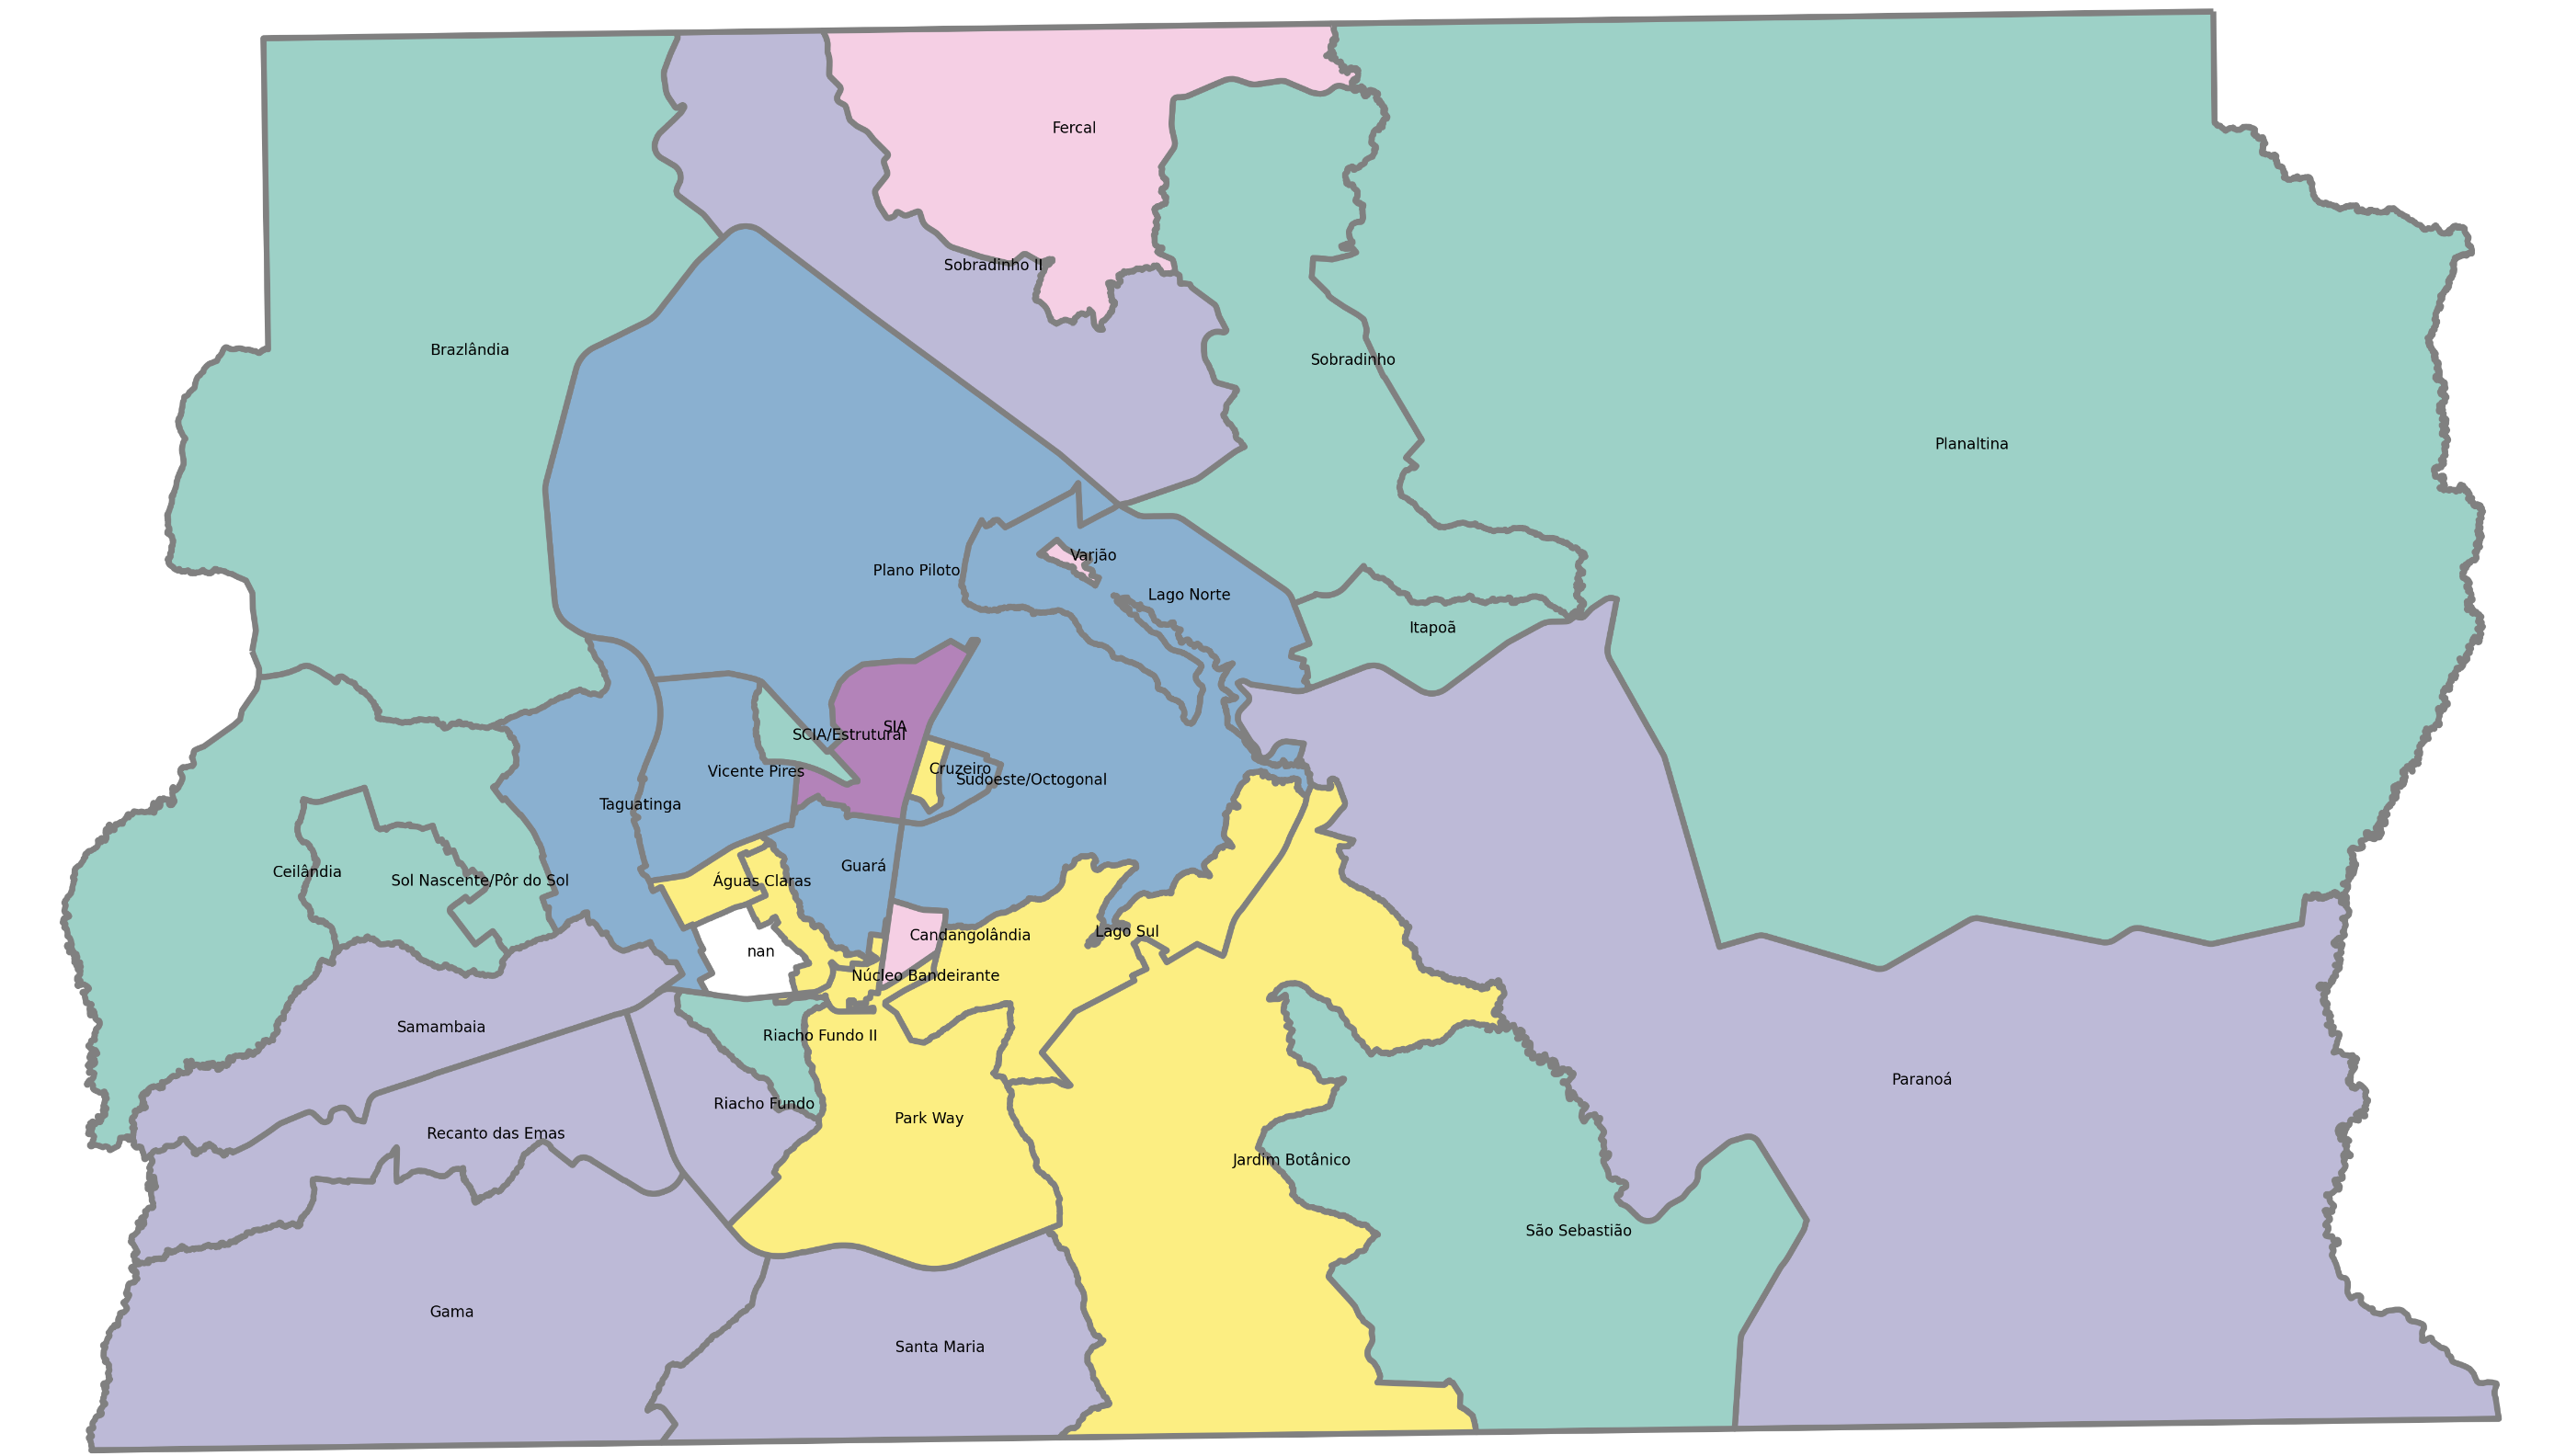
\includegraphics[width=\textwidth]{mapa.png}
  \caption{Clusters Map}
  \label{fig:mapa_cluster}
\end{figure*}

% A partir de uma perspectiva socioeconômica, a formação desses grupos e suas pontuações médias intracluster oferecem um retrato muito lúcido das disparidades regionais, e conseguiu segmentar cidades com nível de vulnerabilidade semelhante.

\subsection{Evaluation of the proposed index within the internal audits published in 2022}

As another tool to assess the proposed index, we compiled all the internal audits reports published in 2022. If the audit was related to one or more Administrative Regions, we noted its service order and respective region, as listed in the table \ref{tab:auditorias-2022}.

When cross-evaluating the data presented in tables \ref{tab:vulnerabilidade} and \ref{tab:auditorias-2022}, we observed that the audit reports dealt with 5 of the top 10 Administrative Regions ranked according to our proposed index. When we evaluated this concordance regarding clusters, the first cluster - composed only of \textit{SIA} - would be audited, the second biggest average risk (cluster 5) would have 1 out of 3 Administrative Regions audited, and the third cluster would have have 6 out of 9 Administrative Regions audited.


\begin{table}[H]
\centering
\begin{tabular}{l|l}
\hline
Service Order & Administrative Region \\
\hline
\centering
109 & Fercal \\
108 & Itapoã \\
104 & Cruzeiro \\
101 & SIA \\
100 & Brazlândia \\
98 & SCIA/Estrutural \\
96 & Gama \\
82 & Plano Piloto \\
82 & Riacho Fundo II \\
79 & Plano Piloto \\
74 & Samambaia \\
74 & Ceilândia \\
74 & Lago Norte \\
74 & Núcleo Bandeirante \\
69 & Gama \\
69 & Santa Maria \\
69 & Plano Piloto \\
63 & Jardim Botânico \\
56 & Sobradinho \\
42 & Paranoá \\
36 & Guará \\
32 & Plano Piloto \\
32 & Guará \\
32 & SIA \\
28 & Plano Piloto \\
28 & SIA \\
21 & Santa Maria \\
19 & Sobradinho II \\
17 & Recanto das Emas \\
9 & Lago Norte \\
\end{tabular}
\label{tab:auditorias-2022}
\caption{Internal audit reports that dealt with audit objects pertaining to one or more Administrative Regions}

\end{table}


\section{Limitations and Conclusions}

This study has its more direct limitation in the facts that Administrative Regions do not have the same statuses as municipalities in the Brazilian constitutional ordination: they do not have executive - in particular budgetary - independence to decide to what ends they will direct their efforts. An Administrative Region can't decide, for example, that it needs a new elementary school: this would have to be proposed by the Federal District's Secretary of Education. A similar conclusion applies to endeavours in all other vulnerabilities we considered here. 

Still, we proposed an index that had a 50\% concordance with what was, as a matter of fact, audited by the government internal auditors. Even though the reports used for our evaluation are not exclusively of internal audits that were planned during the planning phases, this suggests what an application of our vulnerability index would incur in a planning that was at least half the time in accordance to what is currently done.

At last, but not least, we would like to thank the internal auditors Renata Márcia Canuto Dumont and Leandro Shimabukuro for their collaboration with this work.

% \subsection{Aplicabilidade do índice e comparação com as auditorias realizadas entre XXXX - XXXX}
\newpage
\printbibliography
\nocite{*}


\clearpage 
\appendix

\href{https://www.youtube.com/watch?v=5Os2YI8jTr8&ab_channel=EnnioFerreira}{Link para o vídeo no YouTube}

\href{https://github.com/ennioferreirab/case-study-prioritization}{Link para o GitHub}


\begin{longtable}{|c|c|c|c|c|c|c|c|c|c|}
\caption{Consolidated Data} \\
\hline
RA & S1 & S2 & E1 & E2 & E3 & SE1 & SE2 & SEG1 & City \\
\hline
\endfirsthead
\multicolumn{10}{c}%
{{\bfseries \tablename\ \thetable{} -- continued from previous page}} \\
\hline
RA & S1 & S2 & E1 & E2 & E3 & SE1 & SE2 & SEG1 & City \\
\hline
\endhead
\hline
\multicolumn{10}{r}{{Continued on next page}} \\
\hline
\endfoot
\hline
\hline
\endlastfoot
1.0  & -0.841 & -0.131 & -1.511 &  0.176 & -0.197 & -1.357 & -1.200 &  0.537 &             Plano Piloto \\
2.0  & -0.670 & -0.489 & -0.042 & -0.526 & -0.669 &  0.661 & -0.634 & -0.101 &                     Gama \\
3.0  & -0.856 & -0.004 & -0.350 &  0.626 &  0.189 &  0.019 & -0.414 &  0.211 &               Taguatinga \\
4.0  & -0.408 &  2.069 &  0.176 & -0.053 &  0.738 &  0.100 &  0.308 & -0.267 &               Brazlândia \\
5.0  & -0.543 &  2.424 & -0.026 &  1.079 &  2.276 & -0.357 &  0.753 & -0.253 &               Sobradinho \\
6.0  & -0.872 &  0.296 &  1.035 &  1.709 &  1.418 &  1.129 &  0.478 & -0.244 &               Planaltina \\
7.0  & -0.472 & -0.171 &  0.053 & -0.587 & -0.831 &  0.996 &  0.794 &  0.126 &                  Paranoá \\
8.0  &  1.009 & -0.261 &  0.017 &  0.023 &  0.065 & -0.016 & -0.383 &  0.088 &       Núcleo Bandeirante \\
9.0  & -0.964 &  0.571 &  0.649 &  0.855 &  1.039 &  0.048 &  0.714 &  0.142 &                Ceilândia \\
10.0 & -0.704 & -0.480 & -1.467 & -0.220 & -0.112 & -0.811 & -0.813 & -0.222 &                    Guará \\
11.0 &  1.048 &  0.792 &  0.518 & -0.309 & -0.035 & -0.726 & -0.651 & -0.354 &                 Cruzeiro \\
12.0 & -0.881 & -0.331 &  0.270 & -0.587 & -0.522 &  0.284 &  0.570 &  0.032 &                Samambaia \\
13.0 & -0.691 & -0.087 &  1.724 &  0.751 & -0.669 &  0.550 & -0.182 & -0.048 &              Santa Maria \\
14.0 & -0.720 &  0.929 &  0.191 &  0.628 &  0.939 &  1.077 &  1.612 & -0.262 &            São Sebastião \\
15.0 & -0.683 & -0.047 &  1.165 & -1.623 & -0.499 &  1.241 &  0.482 & -0.082 &         Recanto das Emas \\
16.0 &  1.560 & -1.214 &  1.037 & -1.185 & -1.117 & -1.523 & -1.287 & -0.392 &                 Lago Sul \\
17.0 & -0.174 &  1.082 &  0.373 &  2.186 & -0.252 & -0.368 &  0.012 & -0.253 &          Riacho Fundo II \\
18.0 &  0.456 &  0.142 & -1.206 & -0.142 &  1.349 & -1.071 & -1.251 & -0.349 &               Lago Norte \\
19.0 &  1.889 &  0.971 & -1.415 & -0.068 & -0.468 &  0.299 &  0.440 & -0.295 &           Candangolândia \\
20.0 & -0.772 & -0.149 &  1.855 & -0.897 & -0.082 & -1.511 & -1.195 & -0.268 &             Águas Claras \\
21.0 & -0.293 & -1.658 & -0.171 & -2.740 & -1.542 &  0.193 &  0.459 & -0.307 &             Riacho Fundo \\
22.0 &  0.071 & -1.728 & -0.732 & -1.195 & -0.855 & -1.469 & -1.180 & -0.373 &       Sudoeste/Octogonal \\
23.0 &  2.520 & -0.062 & -2.037 & -0.890 & -1.527 &  1.270 &  1.418 & -0.340 &                   Varjão \\
24.0 &  1.858 & -1.231 & -0.348 &  1.450 &  1.727 & -1.486 & -0.858 & -0.432 &                 Park Way \\
25.0 & -0.262 &  0.143 & -0.950 &  1.748 & -0.082 &  1.856 &  2.558 &  0.080 &          SCIA/Estrutural \\
26.0 & -0.534 & -1.270 &  0.054 & -0.042 & -1.628 &  0.463 & -0.280 & -0.358 &            Sobradinho II \\
27.0 & -0.124 & -1.914 &  2.285 & -0.137 &  1.658 & -1.145 & -0.874 & -0.480 &          Jardim Botânico \\
28.0 & -0.489 & -0.752 &  0.687 &  0.059 &  1.302 &  1.077 &  0.451 & -0.012 &                   Itapoã \\
29.0 & -0.191 & -0.052 & -0.991 & -0.145 & -0.715 & -1.084 & -1.020 &  5.427 &                      SIA \\
30.0 & -0.385 &  0.965 & -0.821 & -0.151 & -0.831 & -0.590 & -1.037 & -0.322 &            Vicente Pires \\
31.0 &  2.309 &  1.141 &  0.016 & -0.079 & -0.124 &  1.785 &  0.054 & -0.388 &                   Fercal \\
32.0 & -0.193 &  0.508 & -0.037 &  0.287 &  0.058 &  0.465 &  2.154 & -0.239 &  Sol Nascente/Pôr do Sol \\
\hline
\caption{Consolidated Data} \\
\end{longtable}

\textit{Note: The values of the SE1 variable were multiplied by -1, as they have a 'the higher, the better' relationship, correctly impacting the vulnerability index.}


\end{document}


\end{document}
